%%%%%%%%%%%%%%%%%%%%%%%%%%%%%%%%%%%%%%%%%%%%%%%%%%%%%%%%%%%%%%%%%%%%%%%%%%%%%%%%
%Objetivo: Introduzir os conceitos envolvidos na dissertação bem como do
%trabalho realizado.  A ideia é que qualquer pessoa que leia a introdução
%consiga ter uma visão geral sobre a dissertação.
%Autor: Vagner Clementino<vagnercs@dcc.ufmg.br> e
%		Rodolfo Resende<rodolfo@dcc.ufmg.br>
%Criação: Dom Set 18 22:55:43 BRT 2016
%Modificação: qui mai 11 09:48:42 -03 2017
%Revisão: sáb fev 11 21:18:12 BRST 2017
%%%%%%%%%%%%%%%%%%%%%%%%%%%%%%%%%%%%%%%%%%%%%%%%%%%%%%%%%%%%%%%%%%%%%%%%%%%%%%%%
\chapter{Introdução}
\label{ch:intro}

Dentro do ciclo de vida de um produto de software o processo de manutenção tem
papel fundamental. Devido ao seu alto custo, que segundo alguns estudos varia de
60\% a 90\% do preço final do software~\cite{kaur2015review}, as atividades
relacionadas a manter e evoluir têm sua importância considerada tanto pela
comunidade científica quanto pela indústria. Desde o final da década de
1970~\cite{Zelkowitz:1979:PSE:578504} uma atenção tem sido dada para os custos
da Manutenção de Software. Nas décadas de 1980 e 1990 alguns estudos propuseram
modelos de mensuração do valor necessário para manter o
software~\cite{Herrin:1985:SMC:323287.323383,hirota1994approach}. Apesar da
evolução das metologias para se manter um software a estimativa é que nas
últimas duas décadas o custo de manutenção tenha aumentado em
50\%~\cite{koskinen2010software}. Esta tendência pode ser observada na
Figura~\ref{fig:software-maintence-costs} onde é possível verificar a evolução
dos gastos com manutenção de software como fração do preço final do produto.

\begin{figure}[htpb]
\centering
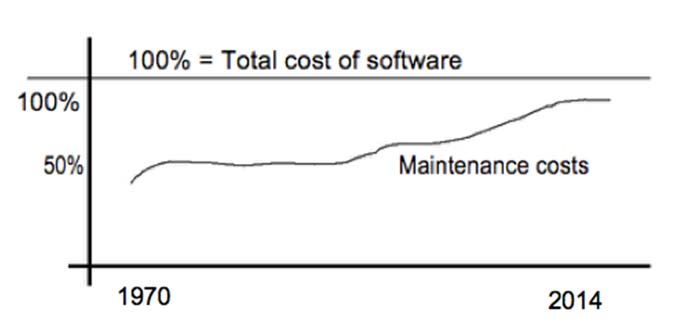
\includegraphics[width=0.6\linewidth]
				{./chapter-intro/img/software-maintence-costs.png}
\caption{Evolução da manutenção de software como percentual do custo total.
	Extraído de~\cite{engelbertink2010save}}
\label{fig:software-maintence-costs}
\end{figure}

Uma vez que o software entra em operação, anomalias são descobertas, mudanças
ocorrem no ambiente de operação e novos requisitos são solicitados pelo usuário.
Todas estas demandas devem ser solucionadas pela Manutenção de Software que se
inicia com entrega do sistema. Contudo, alguns autores defendem que certas
atividades, como aquelas relativas à analise da qualidade, começam bem antes da
entrega do produto.

A \textit{Manutenção}, dentre outros aspectos, corresponde ao processo de
modificar um componente ou sistema de software após a sua entrega com o objetivo
de \textit{corrigir falhas, melhorar o desempenho ou adaptá-lo devido à mudanças
	ambientais}~\cite{{159342}}. De maneira relacionada,
\textit{Manutenibilidade} é a propriedade de um sistema ou componente de
software em relação ao grau de \textit{facilidade} que ele pode ser corrigido,
melhorado ou adaptado~\cite{{159342}}.

% Verificamos na literatura uma discussão sobre a diferença entre manutenção e
% evolução de software. Percebe-se ainda que pesquisadores e profissionais
% utilizam evolução como o substituto preferido para
% manutenção~\cite{Bennett:2000:SME:336512.336534}. Todavia, não está no escopo
% desta dissertação discutir e apresentar as diferenças entre os conceitos. Neste
% sentido, utilizamos os termos \textit{manter} e \textit{evoluir} software de
% forma intercambiáveis.

As manutenções em software podem ser divididas em \textit{Corretiva, Adaptativa,
    Perfectiva e Preventiva}~\cite{Lientz:1980:SMM:601062,159342}. A ISO 14764
discute os quatro tipos e propõe que exista um elemento comum denominado
\textit{Requisição de Mudança (RM)} que representa as características
compartilhadas pelos demais tipos.

\begin{figure}[hbtp] \centering 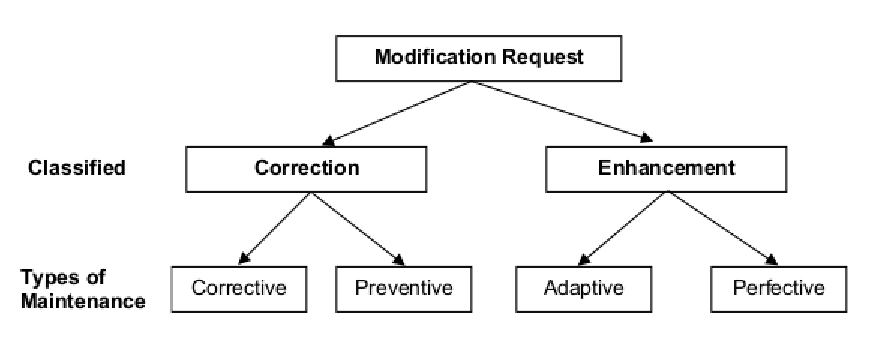
\includegraphics[width=.75\textwidth]
	{./chapter-intro/img/modification_request.eps} \caption{Tipos de manutenção
		segundo a norma ISO/IEC 14764. Extraído de~\cite{1703974}}
\label{fig:modification-request} \end{figure}

Por conta do volume das RM é importante a utilização de um software com o
objetivo de gerenciá-las. Esse controle é geralmente realizado por
\textit{Ferramentas de Gerenciamento de Requisição de Mudança -~FGRM}, que
auxiliam os desenvolvedores na correção de forma individual ou colaborativa de
falhas (bugs) e no desenvolvimento de novas funcionalidades, por exemplo. Estas
ferramentas podem ainda ser utilizadas por gestores, analistas de qualidade e
usuários finais para atividades como gerenciamento de projetos, comunicação,
discussão e revisões de código. A literatura em Manutenção de Software não
define uma nomenclatura comum para este tipo de ferramenta. Em alguns estudos é
utilizado nomes como Sistema de Controle de Defeito -~Bug Tracking Systems,
Sistema de Gerenciamento da Requisição -~Request Management System, Sistemas de
Controle de Demandas (SCD)- Issue Tracking Systems. Todavia, de modo geral, o
termo se refere as ferramentas utilizadas pelas organizações para \textit{gerir
    as Requisições de Mudança}. Neste trabalho utilizaremos o termo
\texttt{Ferramentas de Gerenciamento de Requisições de Mudança} (FGRM) ao
referimos a este tipo de software. A Tabela~\ref{tab:exemplo} apresenta alguns
exemplos de software que podem ser classificados como FGRMs. Também são listados
serviços da Internet que oferecem funcionalidades presentes nas FGRMs na forma
de Software como Serviço~\cite{fox2013engineering}.

\begin{table}[htpb]
\centering
\resizebox{\textwidth}{!}{%
\begin{tabular}{@{}clll@{}}
\toprule
\multicolumn{2}{c|}{Ferramentas}                   & \multicolumn{2}{c}{Serviços da Internet} \\ \midrule
Bugzilla & https://www.bugzilla.org/               & SourceForge  & https://sourceforge.net/  \\ \midrule
MantisBT & https://www.mantisbt.org/               & Lauchpad     & https://launchpad.net/    \\ \midrule
Trac     & https://trac.edgewall.org/              & Code Plex    & https://www.codeplex.com/ \\ \midrule
Redmine  & www.redmine.org/                        & Google Code  & https://code.google.com/  \\
Jira     & https://www.atlassian.com/software/jira & GitHub       & https://github.com/       \\ \bottomrule
\end{tabular}%
}
\caption{Exemplos de ferramentas e serviços da Internet. Extraído
		de~\cite{cavalcanti2014challenges}}
\label{tab:exemplo}
\end{table}

\section{Motivação}
\label{sec:intro-motivacao}

Diante da maior presença de software em todos os setores da sociedade existe um
interesse por parte da academia e da industria no desenvolvimento de processos,
técnicas e \textit{ferramentas} que reduzam o esforço e o custo do
desenvolvimento e manutenção de software. Um exemplo é o trabalho de Yong \&
Mookerjee~\cite{1423995} que propõe um modelo que reduz os custos de manutenção
e reposição durante a vida útil de um sistema de software. O modelo demonstrou
que em algumas situações é \textit{melhor substituir um sistema do que
    mantê-lo}.  Este pro\-ble\-ma é agravado tendo em vista que em alguns casos
são necessários 60\% dos desenvolvedores dedicados à tarefas de manutenção de
sistemas~\cite{Zhang_2003}.

Dependendo do tamanho de um projeto de software é necessário a utilização de uma
FGRM para gerenciar as Requisições~de~Mudança por conta do volume e das
diferentes partes interessadas que necessitam de um local centralizado onde
possa registrar as falhas encontradas e as melhorias que
necessitam~\cite{1407819}. Neste sentido, podemos afirmar que as RMs suportam
projetos de diferentes tipos e tamanhos, sejam eles de código aberto (Apache,
Linux, Open Office) ou em organizações públicas e privadas (NASA e IBM). Dando
suporte à software de diferentes plataformas, seja aplicativos de área de
trabalho (desktop), web ou móvel (mobile).

A literatura da área nos mostra que as FGRMs desempenham um papel além do
gerenciamento dos pedidos de manutenção software. Avaliando o controle de
demandas como um processo social, Bertram e
outros~\cite{Bertram:2010:CCB:1718918.1718972} realizaram um estudo qualitativo
sobre FGRMs que são utilizadas por equipes pequenas de desenvolvimento de
software. Os resultados demonstraram que a ferramenta não é apenas um banco de
dados de rastreamento de falhas, mas atua como um ponto central para a
comunicação e coordenação de diversas partes interessadas (stakeholders) dentro
e fora da equipe de manutenção. Os clientes, gerentes de projeto, analistas de
qualidade e programadores contribuem em conjunto para o compartilhamento de
conhecimento do projeto por meio da utilização das FGRMs.

No trabalho de Breu e outros~\cite{Breu:2010:INB:1718918.1718973} o foco é
analisar o papel dos FGRMs no suporte à colaboração entre desenvolvedores e
usuários de um software. Com base nos resultados foi possível verificar que o
uso da ferramenta possibilitou que os usuários desempenhassem um papel além de
simplesmente reportar uma falha: a participação ativa e permanente foi
importante no progresso da resolução das falhas que eles descreveram.

Um outro benefício da utilização das FGRM é que as mudanças no
software podem ser rapidamente identificadas e reportadas para os
desenvolvedores~\cite{anvik2005coping}. Além disso, eles podem ajudar a estimar
o custo do software, na análise de impacto, planejamento, rastreabilidade,
descoberta do conhecimento~\cite{cavalcanti2013bug}.

Conforme exposto as FGRMs desempenham um papel fundamental no contexto do
desenvolvimento e manutenção de software. Contudo, no escopo de utilização das
FGRMs diversos desafios se apresentam: duplicação de RMs, pedidos de modificação
abertos inadvertidamente, grande volume de RMs que devem ser atribuídas aos
desenvolvedores mais aptos, erros descrito de forma incompleta, análise de
impacto das RMs e atribuídas de maneira
incorreta~\cite{cavalcanti2014challenges}. Diante destes problemas e desafios é
importante entender como estas ferramentas estão sendo utilizadas. Com base
neste conhecimento, e com  o que está sendo proposto na literatura, é possível
avaliar e entender necessidades dos profissionais envolvidos com Manutenção de
Software com o objetivo de melhorar as funcionalidades oferecidas por este tipo
de software.

%No trabalho de Junio et al.~\cite{5741246} é proposto um processo denominado
%PASM (Process for Arranging Software Maintenance Requests) que propõe lidar com
%tarefas de manutenção como projetos de software. Para tanto, utilizou-se
%técnicas de análise de agrupamento (clustering) a fim de melhor compreender e
%comparar as demandas de manutenção. Os resultados demostraram que depois de
%adotar o PASM os desenvolvedores tem dedicado um tempo maior para análise e
%validação. De outra forma, relacionada um menor tempo foi dedicado às tarefas
%de execução e codificação.
%
%No estudo realizado por Bettenburg et al.~\cite{bettenburg2008makes} foi
%desenvolvida uma pesquisa (\textit{survey}) entre desenvolvedores e usuários
%dos projetos Apache\footnote{\url{http://www.apache.org/}},
%Eclipse\footnote{\url{https://www.eclipse.org}} e
%Mozilla\footnote{\url{https://www.mozilla.org}} a fim de verificar o que
%produziria uma boa FGRM\@. Os resultados demonstraram que do ponto de vista dos
%desenvolvedores eram consideradas úteis funcionalidades tais como reprodução do
%erro, rastros de pilhas (stack traces) e casos de testes. A partir deste
%resultado foi construído um protótipo capaz de conduzir os usuários na coleta e
%fornecimento de um maior número de informações úteis para a resolução do
%defeito reportado.
%
%
%Em Zimmermann et al.~\cite{5070993} é discutido a importância de que a
%informação descrita em uma Requisição de Mudança seja relevante e completa a
%fim de que o defeito reportado seja resolvido rapidamente. Contudo, na prática,
%a informação apenas chega ao desenvolvedor com a qualidade requerida após
%diversas interações com o usuário afetado. Com o objetivo de minimizar este
%problema os autores propõe um conjunto de diretrizes para a construção de um
%ferramenta capaz de reunir informações relevantes a partir do usuário e
%identificar arquivos que precisam ser corrigidos para resolver o defeito.
%

%No trabalho de Kononenko et al.~\cite{Kononenko:2014:DED:2591062.2591075} é
%apresentada uma ferramenta denominada \textit{DASH} cujo objetivo é agrupar as
%demandas que são relevantes para as atividades de um desenvolvedor.
%Naturalmente todas as demandas ditas relevantes deveriam estar sob a
%responsabilidade de um mesmo programador. O principal objetivo desta ferramenta
%é aumentar a Consciência Situacional (Situational Awareness) dos
%desenvolvedores. Segundo os autores, o principal ganho do uso da ferramenta é
%que os programadores podem gerenciar melhor o excesso de informação e ficar
%mais ciente da evolução das demais demandas do sistema.
%
%Na ferramenta proposta por Thung et al.~\cite{Thung:2014:DIT:2642937.2648627} o
%foco é na determinação de defeitos duplicados. A contribuição deste trabalho é
%a integração do estado da arte de técnicas não supervisionadas para detecção de
%falhas duplicadas conforme proposto por Runeson et
%al.~\cite{Runeson:2007:DDD:1248820.1248882}. A ferramenta utiliza o Modelo de
%Vetor Espacial (Vetor Space Model) como métrica de similaridade entre os
%defeitos e fornece aos desenvolvedores uma lista de possíveis duplicatas.

%A manutenção não necessariamente exige que o processo de software envolvido
%seja o tradicional. Percebe-se alguns exemplos de adoção das práticas ágeis
%para fins de manutenção e evolução do software~\cite{kajko2009model,
%Heeager2015, Devulapally2015,Naz2016}. Tal tendência não é surpreendente tendo
%em vista que os métodos ``ágeis'' enfatizam características úteis à eficiência
%da implementação de software, tais como desenvolvimento incremental e teste
%contínuo que agregam valor para a evolução e manutenção eficaz de um sistema
%\cite{thomas2006agile}. Dentro desta tendência verifica-se a necessidade de que
%as ferramentas envolvidas no suporte à manutenção de software se adéquem à este
%nova forma de manter software.
%

\section{Problema}
\label{sec:intro-problema}

O desenvolvimento e a manutenção de software envolvem diversos tipos de métodos,
técnicas e ferramentas. Em especial no processo de Manutenção, um importante
aspecto são as diversas RMs que devem ser gerenciadas. Este controle é realizado
pelas FGRMs cujo o uso vem crescendo em importância, sobretudo, por sua
utilização por gestores, analistas da qualidade e usuários finais para
atividades como tomada de decisão e comunicação. Contudo, em alguns casos, as
ferramentas são meramente interfaces melhores para o banco de dados que
armazena as RMs~\cite{zimmermann2009improving}. Apesar da inegável importância
das FGRMs, percebe-se um aparente desacoplamento deste tipo de ferramenta com as
necessidades das diversas partes interessadas (stakeholders) na manutenção e
evolução de software. A utilização de \textit{``demanda''} como conceito central
para as FGRMs parece ser distante das necessidades práticas dos projetos de
software, especialmente no ponto de vista dos desenvolvedores
\cite{Baysal:2013:SAP:2486788.2486957}.

Um exemplo deste desacoplamento pode ser visto no trabalho proposto por Baysal
\& Holme~\cite{baysal2012qualitative} no qual desenvolvedores que utilizam o
Bugzilla\footnote{\url{https://www.bugzilla.org}} relataram dificuldade em
manter uma compreensão do escopo que as RMs atribuídas a eles possuem. Segundo
os participantes do estudo seria importante que a ferramenta tivesse um suporte
melhorado para o conceito de Consciência Situacional~-~Situational Awareness. Em
síntese, eles gostariam de estar cientes da situação global do projeto bem como
das atividades que outras pessoas estão realizando.

Existem outros prolemas que são potencializados pela ausência de certas
funcionalidades nas FGRMs. Um exemplo são as RMs que acabam sendo relatadas com
baixa qualidade. Nesta situação os usuários acabam sendo questionados a inserir
mais detalhes que muitas vezes eles não tem conhecimento. Por outro lado,
verifica-se uma frustração por parte dos desenvolvedores que acabam desapontados
sobre a qualidade do que foi reportado~\cite{just2008towards}.

Corroborando com a necessidade de evolução das FGRMs, o estudo realizado por
Zimmermann e outros~\cite{zimmermann2009improving} propõem quatro dimensões de
melhorias para este tipo de software. Estas dimensões estão apresentadas na
Figura~\ref{fig:dimensoes_melhorias_fgrm} e serão detalhadas no
Capítulo~\ref{ch:mapeamento-sistematico} onde foram utilizadas na classificação
de estudos no Mapeamento Sistemático realizado.

% \begin{enumerate} [(i)]
% 	\item{Informação}
% 	\item{Processo}
% 	\item{Usuário}
% 	\item{Ferramenta}
% \end{enumerate}

\begin{figure}[htpb] \centering
	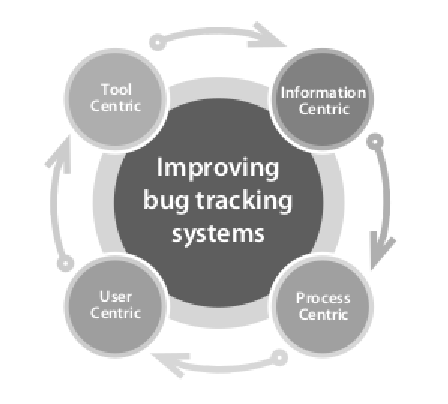
\includegraphics[width=0.6\linewidth]
	{chapter-intro/img/dimensoes_melhorias_fgrm.pdf}
	\caption{Dimensões de melhoria das FGRMs. Extraído de~\cite{zimmermann2005mining}}
\label{fig:dimensoes_melhorias_fgrm}
\end{figure}

Neste estudo estamos especialmente interessados em analisar e propor melhorias
relativas ao domínio da \textit{Ferramenta}. Ao bem do nosso conhecimento é
reduzido o número de trabalhos que avaliem de forma sistemática as
funcionalidades oferecidas pelas FGRMs ao mesmo tempo que faça relação com que
vem sendo proposto na li\-te\-ra\-tu\-ra sobre o assunto.

É importante ressaltar que os estudos sobre melhorias das FGRMs a crescente
adoção de técnicas propostas pelos agilistas na Manutenção de
Software~\cite{Soltan2016,Devulapally2015, Heeager2015}. Neste contexto, seria
importante que ferramentas que dão suporte à manutenção, tal como as FGRMs,
evoluíssem para se adaptar a esta nova forma de trabalhar. Um outro fator que
agrega sobre a necessidade de adequação das FGRMs são as diversas extensões
(plugins) propostas na literatura
\cite{101186,Thung:2014:BIT:2635868.2661678,Kononenko:2014:DED:2591062.2591075}.

\section{Objetivos}
\label{sec:intro-objetivos}

Segundo o nosso entendimento existe um distanciamento entre as necessidades dos
profissionais envolvidos em Manutenção de Software e as funcionalidades
oferecidas pelas FGRM\@. Por esta razão este trabalho de dissertação investiga e
contribui no entendimento de como as Ferramentas de Gerenciamento de Requisição
de Mudança estão sendo melhoradas ou estendidas no contexto da transformação do
processo de desenvolvimento e manutenção de software de um modelo tradicional
para outro que incorpora cada vez mais as práticas propostas pelos agilistas. O
intuito é analisar como as FGRM estão sendo modificadas com base na literatura
da área em contraste com o ponto de vista dos profissionais envolvidos em
manutenção de software.

Neste contexto, elaboramos um estudo sobre as Ferramentas de Gerenciamento de
Requisição de Mudança (FGRM) com os seguintes objetivos:
\begin{enumerate}[(i)]
	\item entender os requisitos comuns deste tipo de ferramenta;
	\item mapear as melhorias para as FGRM que estão sendo propostas na
		literatura;
	\item avaliar sobre o ponto de vista dos profissionais a
		situação atual dos FGRM\@;
	\item propor melhorias ou novas funcionalidades para as FGRM\@.
\end{enumerate}

%Vamos discutir os aspectos que são considerados mais importantes a partir da
%literatura da área, bem como do ponto de vista de profissionais envolvidos em
%manutenção de software. De forma particular, iremos estudar os mecanismos de
%personalização que algumas destas ferramentas permitem e tentaremos ainda criar
%exemplos de personalização para alguma possível extensão a ser identificada ao
%longo do trabalho.

\section{Visão Geral da Dissertação}
\label{sec:intro-visao-geral}

A fim de alcançarmos os objetivos descritos foi proposto um conjunto de
melhorias para as funcionalidades das FGRMs. As melhorias foram realizadas com
base em três estudos empíricos: um mapeamento sistemático da literatura,
apresentado no Capítulo~\ref{ch:mapeamento-sistematico}; e uma pesquisa com
profissionais, apresentada no Capítulo~\ref{ch:pesquisa-profissionais}; um
levantamento com questionário validando sugestões de melhorias descrito no
Capítulo~\ref{ch:sug_melhoria}.

Mediante o mapeamento sistemático obtivemos e avaliamos o estado da arte sobre
novas funcionalidades que estão propostas na literatura. A partir do estudo foi
possível propor dois esquemas de classificação: por dimensão de melhoria e
suporte ao papel desempenhado na manutenção de software. De maneira similar,
através da caracterização das funcionalidade de algumas FGRMs código aberto ou
disponíveis comercialmente e escolhidas mediante uma pesquisa com profissionais
identificamos o estado da prática deste tipo de ferramenta.

Com base em dois estudos anteriores conduzimos uma pesquisa com profissionais
envolvidos em manutenção de software onde pedimos que avaliassem os requisitos
funcionais e não funcionais que poderiam melhorar as FGRM já existentes. O
questionário também quis saber a opinião dos profissionais sobre a relevância
das propostas de me\-lho\-ri\-as existente na literatura em sua rotina de
trabalho. Fundamentado nos estudos descritos foi proposto um conjunto de
melhorias.  Como prova de conceito, uma destas melhorias foi implementada como
uma extensão de uma FGRM\@.

\section{Metodologia de Pesquisa}
\label{sec:intro-metodologia}

A metodologia de pesquisa utilizada neste estudo é baseada em uma abordagem
multi-método~\cite{hesse2010mixed}. Este tipo de desenho combina dois ou mais
métodos quantitativo (ou qualitativo) em um único estudo. Um estudo que faça uso
de um survey e um experimento é um exemplo deste tipo de
enfoque~\cite{hesse2010mixed}.

% Alguns estudos descrevem quatro tipos de desenho em abordagens multi-método:
% embutido (embedded), exploratória, triangulada e
% explanatória~\cite{creswell2007designing}. Neste estudo, utilizamos uma
% abordagem de triangulação no qual consolidamos os resultados de diferentes
% métodos, considerando, contudo, que a mesma questão de pesquisa foi investigada
% em cada um deles. A utilização de um desenho triangular no trabalho melhora as
% conclusões e completude do estudo, trazendo maior credibilidade para os achados
% da pesquisa~\cite{hesse2010mixed}.

As etapas do trabalho, que compõem a abordagem multi-método estão listadas a
seguir:

\begin{itemize}[(i)]
	\item Mapeamento Sistemático da Literatura~\cite{Petersen2008}
	\item Caracterização das Ferramentas de Gerenciamento de Requisição de
		Mudança (FGRM)
	\item Pesquisa (Survey) com os
		desenvolvedores~\cite{wohlin2012experimentation}
%	\item Desenvolvimento de extensões para as FGRMs
\end{itemize}

\section{Contribuições do Estudo}
\label{sec:intro-contribuicao}

Este estudo sistematiza a literatura sobre melhorias das funcionalidades das
FGRMs ao mesmo tempo que avalia junto aos profissionais as relevâncias de tais
alterações. Este estudo ainda se propõe este tipo de software por meio de uma
caracterização de suas funcionalidades. Ao final deste trabalho teremos um
conjunto de funcionalidades que podem ser implementadas neste tipo de software
visando a sua melhoria.

\section{Organização do Trabalho}
\label{sec:intro-organizacao-dissertacao}

Este trabalho de dissertação está organizado conforme descrito a seguir. No
Capítulo~\ref{ch:visao-geral-manutencao} apresentamos e discutimos os principais
conceitos neste estudo. Neste mesmo capítulo é descrito um estudo onde coletamos
as principais funcionalidades de um conjunto de FGRMs que foram definidas como
relevantes na visão de profissionais envolvidos em Manutenção de Software.

Um Mapeamento Sistemático da Literatura foi conduzido no
Capítulo~\ref{ch:mapeamento-sistematico} com o objetivo de levantar as melhorias
nas funcionalidades das FGRMs que estão sendo propostas na literatura. Os
estudos foram classificados em dimensões de melhorias e pelo papel desempenhado
na Manutenção de Software que a melhoria visa dar suporte.

No Capítulo~\ref{ch:pesquisa-profissionais} reunimos a opinião de profissionais
envolvidos em Manutenção de Software sobre as funcionalidades oferecidas pelas
FGRMs que eles utilizam. Estes profissionais exercem suas atividades em projetos
de código aberto e empresas no setor público e privado. Foi possível identificar
que grande parte dos profissionais estão satisfeito com a ferramenta que
utiliza, contudo, eles estão bastante interessados em novos tipos de
comportamento no software.

Tomando como base a literatura sobre melhorias nas FGRMs e os resultados obtidos
nos estudos descritos nos capítulos anteriores, apresentamos e discutimos um
conjunto de sugestões de melhorias no Capítulo~\ref{ch:sug_melhoria}. As
recomendações propostas foram avaliadas por profissionais que contribuem no
desenvolvimento de FGRM\@. Em geral, as recomendações tiveram boa aceitação
tanto sobre sua necessidade quanto por sua facilidade de implementação.  No
Capítulo~\ref{ch:implemtacao_extensao} foi realizada uma prova de conceito uma
das sugestões propostas foram implementadas com uma extensão de uma FGRM\@. As
conclusões e trabalhos futuros estão descritos no
Capítulo~\ref{ch:conclusao_trab_futuros}.
